\documentclass[11pt]{report}
\usepackage[utf8]{inputenc}
\usepackage[mieic]{feupteses}
\usepackage{color}
\usepackage[english]{babel}
\usepackage{dirtytalk}
\usepackage{titlesec}
\usepackage{epigraph}
\usepackage{multicol}
\usepackage{wrapfig}
\usepackage{xcolor}
\usepackage{framed}
\usepackage{pdflscape}
\definecolor{shadecolor}{RGB}{180,180,180}
\definecolor{cloudwhite}{cmyk}{0,0,0,0.025}
\graphicspath{{figures/}}

\newcommand{\TODO}[1]{
	 \textcolor{red}{#1}
}

\newenvironment{pattern}[1]{
  \section{#1}
  \newcommand{\context}[1]{
  \begin{snugshade*}\noindent\textsc{Context} \end{snugshade*}
    ##1
    }
  \newcommand{\problem}[1]{
    \begin{snugshade*}\noindent\textsc{Problem} \end{snugshade*}
    ##1
  }
  \newcommand{\forces}[1]{
    \begin{snugshade*}\noindent\textsc{Forces} \end{snugshade*}
    ##1
  }
  \newcommand{\solution}[1]{
    \begin{snugshade*}\noindent\textsc{Solution} \end{snugshade*}
    ##1
  }
  \newcommand{\rationale}[1]{
    \begin{snugshade*}\noindent\textsc{Rationale} \end{snugshade*}
    ##1
  }
	\newcommand{\related}[1]{
		\begin{snugshade*}\noindent\textsc{Related Patterns} \end{snugshade*}
		##1
	}
}

\newenvironment{companyreport}[1]{

  \subsection*{#1}
  \newcommand{\product}{
  \begin{snugshade*}\noindent\textsc{Product} \end{snugshade*}
  }
  \newcommand{\teams}{
    \begin{snugshade*}\noindent\textsc{Teams} \end{snugshade*}
  }
  \newcommand{\development}{
    \begin{snugshade*}\noindent\textsc{Development} \end{snugshade*}
  }
  \newcommand{\operations}{
    \begin{snugshade*}\noindent\textsc{Operations \& Infrastructure Management} \end{snugshade*}
  }
	\newcommand{\reportend}{
		\pagebreak
	}
}

\begin{document}

	\title{Towards DevOps: \\ Practices and Patterns from the Portuguese Startup Scene }
	\author{Carlos Manuel da Costa Martins Teixeira}
	\supervisor{Supervisor}{Prof. Hugo Sereno Ferreira}
	\supervisor{Co-Supervisor}{Tiago Boldt Sousa}
	\logo{uporto-feup.pdf}
	\additionalfronttext{Dissertation}

\begin{Prolog}
  \chapter*{Abstract}

Software and its development have been increasing both in complexity and in size. As more businesses were moving first to the Internet and then to the Cloud, new technologies and opportunities started to emerge. As the environment were they acted changed, most practices and mindesets stayed the same causing a imbalance between the external and internal environment of companies. In the midst of this confusion new ideas started to appear with the objective of restoring the balance between the environment and those who operated eventually culminating in the rise of DevOps.

But what is DevOps? Formed by combining the word Development with the word Operations, the word  "DevOps" has been around for sometime. Uses and appearances have been seen in different contexts and with different meanings making it a topic of discussion and discord. Being mostly refered to as a movement aiming to conciliate Software Operations and Software Developer professionals, there are those who see it as no more than a set of tools or a new job position. This mismatch of interpretations and overall lack of understanding of DevOps often means that companies and professionals lack the knowledge to fully take advantage of the benefits that DevOps brings. 

In this thesis we demystify and formalize DevOps, first by using the existing literature as a basis to create a DevOps state-of-the-art and then by analysing the current practices associated with DevOps in the real world. The analysis, done by interviewing and observing some startups from Portugal is then the basis from wich we then extract a set of patterns related with DevOps and its values. Some of the 13 identified patterns are then validated by watching the effects of the DevOps culture in real people in real world situations.

In the end we conclude that even though the collected information allows us to have some knoledge and grasp of DevOps and its broad scope, due to that same broad scope more work and investigation is needed in order to fully understand the movement and its consequences.
  \pdfbookmark[0]{Table of Contents}{contents}
  \tableofcontents
  \cleardoublepage
  \pdfbookmark[0]{List of Figures}{figures}
   \listoffigures
   \cleardoublepage
   \pdfbookmark[0]{List of Tables}{tables}
   \listoftables
   \chapter*{Abbreviations}
\chaptermark{ABBREVIATIONS}

\begin{flushleft}
\begin{tabular}{l p{0.8\linewidth}}
ADT      & Abstract Data Type\\
NIST     & National Institute of Standards and Technology\\
SaaS     & Software as a Service\\
PaaS     & Platform as a Service\\
IaaS     & Infrastructure as a Service\\
\end{tabular}
\end{flushleft}

  % the list of abbreviations used
\end{Prolog}


\StartBody

\chapter{Introduction} \label{chap:introduction}

	\section{Context} \label{chap:introduction:sec:context}

		As the Internet grew and more people joined, an ever increasing number of
	businesses and opportunities started to emerge.
		
	    Initially, businesses that wanted to provide services over the Internet would need to buy servers, hire operations crews and buy real estate to accommodate the previous two. Additionally, businesses were also subjected to large usage fluctuations. This meant that a lot of the time, servers and teams were not being used in an optimal way. 
	    
	    Large upfront costs combined with large maintenance costs and unused resources were obviously not desirable and eventually solutions to this problems started to appear. Eventually named ”cloud computing”, the solution consisted in a new type of business that allowed other businesses to rent computing resources with little to no upfront costs. Cloud computing providers would charge businesses based on the usage as well as allow them to quickly increase or decrease computing resources. This elasticity combined with the elimination of the previously mentioned upfront costs meant that more businesses could be born and that the existing ones could lower their operational costs.

		In the midst of this change a new set of opportunities and problems started to arise. This ideas and problems eventually started the denominated DevOps movement. This movement called for the end of organizational boundaries between operations and development departments, integration of the previous two and the automation of repetitive tasks. This way DevOps aimed to reduce software time to market, teams sizes and also increase businesses agility and efficiency.	

	\section{Problem} \label{chap:introduction:sec:problem}

		The DevOps movement spans throughout a vast set of areas. This means that successfully understanding DevOps is not easy and can often seem like a never ending task requiring an informed and multidisciplinary approach.

		Regarding the current state of the literature on DevOps there is not a lot of investigation done on the subject \ref{chap:stateoftheheart:sec:devops:challenges}. 

		Companies that want do adopt DevOps are, as a result, required to learn the challenges and solutions of adopting DevOps while adopting it. Obviously this is far from being ideal and consequently companies may fail to adopt DevOps or practice it in an efficient way.

		   
	\section{Motivation \& Objectives} \label{chap:introduction:sec:motivation}

	    This work aims to provide companies and teams that want to adopt DevOps with knowledge relative to DevOps and the adoption process. This information should be easy to access and understand and, it should allow companies to have a feeling of the effort needed to adopt DevOps as well as allow them to define a preliminary road map for the adoption. 
	    
	    Lastly with the information provided, companies must be able to solve most of the problems that will appear when adopting DevOps.

    \section{Expected Contributions} \label{chap:introduction:sec:contributions}

    	Contributions of this work will be:
    	\begin{itemize}
    		\item{A comprehensive description of the current state of the art regarding the DevOps movement.}
    		\item{Identification of good practices concerning the DevOps adoption.}
    		\item{Elicitation of common obstacles faced when adopting DevOps.}
    		\item{Validation of the former two items in a real world scenario.}
    	\end{itemize}

    \section{Outline} \label{chap:introduction:sec:outline}
    	This report was made as preparation for the dissertation.

    	In it there is a Introduction \ref{chap:introduction}, followed by the state of the art \ref{chap:stateoftheart} regarding the reach and size of the Internet \ref{chap:stateoftheart:sec:internet}, cloud computing \ref{chap:stateoftheart:sec:cloud} and DevOps \ref{chap:stateoftheart:sec:devops}.
    	Section \ref{chap:towardsdevops} defines both the problem \ref{chap:towardsdevops:sec:problem}, the solution \ref{chap:towardsdevops:sec:solutionperspective}, and the methodology \ref{chap:towardsdevops:sec:methodology}.
    	Then, the method for validating the obtained results is described in \ref{chap:validation}.

    	Lastly, the Conclusion is presented and the planning for the future work is presented \ref{chap:conclusion}.  
\chapter{State of The Art} \label{chap:stateoftheart}
DevOps is usually associated with different types of technologies and practices. Effectively applying DevOps means not only to understand the cultural aspects but also the technological aspects that enabled some of its practices.
In this chapter an introduction to cloud computing will be presented providing the needed context for the following section where a brief set of events involved in the rise of DevOps movement will be presented. After this, a small characterization of the Portuguese start-up scene will be presented in order to justify some of the choices presented in the next chapter \ref{chap:towardsdevops:sec:methodology:sec:sample}.

    \section{Cloud Computing} \label{chap:stateoftheart:sec:cloud}

        Paraphrasing \cite{Bass}, imagine  wanting to use electricity. Rather than building an entire grid and a power plant, one only needs to connect to the public network.In the common scenario, charges are calculated based on the usage amount and no special knowledge of how the network setup is needed.

        Clouds follows exactly the same rationale, rather than having to build/purchase the computing resources, one needs only to connect to a provider and the resources are available to be used. Charges, like in the electric grid, are calculated based on the usage and clients do not need to know how the resources are managed or setup.

        \subsection{Definition}
        In \cite{Mell2011}, NIST\footnote{National Institute of Standarts and Technologie} defines Cloud computing as \textit{a model for enabling ubiquitous, convenient, on-demand network access to a shared pool of configurable computing resources (e.g., networks, servers, storage, applications, and services) that can be rapidly provisioned and released with minimal management effort or service provider interaction.}

        NIST also defines the following essential characteristics of cloud computing:

        \begin{itemize}
            \item \textbf{On-demand self-service} : A consumer can unilaterally provision computing capabilities, such as server time and network storage, as needed automatically without requiring human interaction with each service provider.
            \item \textbf{Broad network access} :  Users must be allowed to access resources through standard mechanism.
            \item \textbf{Resource pooling} : A multi-tenant model should be used in order to serve multiple users. Resources are allocated dynamically meaning that users do not know were, physically, the allocated resources are \cite{Garrison2012}
            \item \textbf{Rapid elasticity} : Resources can be elastically allocated or deallocate. This should be possible to be done automatically \cite{Mell2011}
            \item \textbf{Measured service} : The usage of resources should be measured providing transparency in the provider-client relation.
  	    \end{itemize}

        \subsection{Delivery methods} \label{chap:stateoftheheart:sec:cloud:sec:deliverymethods}
          In regards to their accessibility, it is common to identify three main categories of clouds \cite{Zhang2010} :
        	\begin{itemize}
            	\item \textbf{Public Clouds} : Public clouds are a pool of resources hosted by cloud providers who rent them to the general public. This resources can be accessed over the Internet and are shared among users.

    		      \item \textbf{Private Clouds} : Private clouds are usually administered and used by the same organization. Alternatively a third party can also be hired to manage the resources. The main difference between public and private clouds is the usage of the resources. Private clouds resources are only used by one company as opposed to public clouds were resources are shared.

              \item \textbf{Hybrid Clouds} : Hybrid clouds combine both the private and public concepts. When using an hybrid clouds approach, infrastructure is divided by the two types of clouds meaning that some modules may be hosted in the private space and others on the public one.

              \item \textbf{Virtual Private Cloud} : Virtual private clouds are an alternative to private clouds. This type of cloud are essentially a public cloud that \textit{leverages virtual private network (VPN) technology..}\cite{Zhang2010} allowing users to combine characteristics of both public clouds and private clouds.
    		\end{itemize}

      \subsection{Service Levels} \label{chap:stateoftheheart:sec:cloud:sec:servicelevels}
  		In terms of service levels cloud computing can be classified in regard to the provided abstraction. The main categories are the following \cite{Vaquero2008} :
  		\begin{itemize}
  			\item \textbf{SaaS} - Software as a Service (SaaS) gives users access to a platform usually through a web client. Without the need to  download or install software the user is able to use the provided software instantly and virtually everywhere.\linebreak Applications of this model include messaging software, email services, collaborative platforms, etc.
 				\item \textbf{PaaS} - Platform as a Service (PaaS) allows it's users to quickly deploy applications with little to no configuration. In this type of platform environments are usually setup previously or configurable. PaaS users should nevertheless expect only to be able to deploy applications or software supported by the provider.
  			\item \textbf{IaaS} - Infrastructure as a Service (IaaS) represents the lowest abstraction made available by cloud providers. In this model the user is able to configure and access a machine directly without constraints. This machine, usually a virtual server managed by the provider, can be configured and maintained by the user.\linebreak This model is used when applications are complex and therefore need complex configurations.
  		\end{itemize}

  		\subsection{Benefits} \label{chap:stateoftheheart:sec:cloud:sec:benefits}
  			The main advantages of cloud computing for its users can be summarized as following:
  			\begin{itemize}
  				\item \textbf{Monetary Efficiency} - Cloud providers allow users to keep their resources to the needed minimum. By allowing users to quickly and easily increase/decrease the allocated resources amount and billing clients only for the resources used, cloud providers are good way to save money and spend only the needed amount \cite{Garrison2012,Mell2011}.
  				\item \textbf{Scalability} - usually through a public API of some kind most cloud providers allow for the quick increase or reduction of resources \cite{Mell2011}. This enables businesses to quickly go from zero to millions of users with minimum overhead. Additionally because processes related with the management and configuration of cloud servers can be automated it is usually possible to manage large systems with small teams \cite{Loukides2012}.
  	    	\item \textbf{Maintainability} - Cloud Providers are responsible for the maintenance of all the hardware and infrastructure aspects. Cloud computing users therefore do not need to worry about updating the hardware or maintaining the physical infrastructure. This enables users to focus their resources in improving their product rather than improving the structure that supports it \cite{Garrison2012}.
  			\end{itemize}

	\section{DevOps} \label{chap:stateoftheart:sec:devops}
      In \textit{Why DevOps Is Like An Onion} \cite{DaveSayers2013}, Dave Sayers chooses to use the analogy of peeling an onion, with each layer representing a different concept, in order to describe DevOps. Further developing upon his initial idea, in this section, we will try to introduce DevOps using that same analogy.

      \subsection{The cultural layer} \label{chap:stateoftheart:sec:devops:sec:culture}
      Looking at some of the first DevOps efforts we see that a lot of them aimed to create a better articulation between Developers and Operations \cite{Debois2008} \cite{Allspaw}.\\
      Being two distinct departments with different work methodologies and objectives, this meant that some cultural changes had to happen in order for the two departments to be able to create a common understanding of each other worlds \cite{Allspaw}.\\
      The main cultural values associated with DevOps are, as a result, values that promote cooperation and communication. These are some of the ones that we identified:
      \begin{itemize}
          \item Respect \cite{Davis2015} \cite{Allspaw}
          \item Trust \cite{Huttermann2012}
          \item Collaboration \cite{Davis2015}
          \item Sharing \cite{Willis2010}
      \end{itemize}

      \subsection{The methodology layer} \label{chap:stateoftheart:sec:devops:sec:methodology}
      The DevOps movement does not define a specific methodology mostly since it belives that this choice should be made by the company/organization in order to better accomodate their needs. Nevertheless, when we look for instance at CAMS\ref{chap:stateoftheart:sec:devops:sec:definition} or at some of the practices like \textit{Continuous Deployment} it becomes clear that, altough a methodology is not defined, the one chosed should enable an iterative and continuous improvement focused approach.

      \subsection{The practices layer} \label{chap:stateoftheart:sec:devops:sec:practices}
      Broadly speaking, DevOps practices gravitate around the automation of processes. From the setup of environments on the developers machine, up to the deployment phase, the capacity to automate repetitive tasks is a key feature of DevOps.
      Common practices associated with the DevOps movement include:
      \begin{itemize}
        \item \textbf{Continuous Integration} - Regular integration of software helps discover risks associated with the integration with the integration of the software. \cite{And2015}
        \item \textbf{Continuous Deployment} - Deploying often means that less functionalities are deployed each time. This makes deployments more manageable and in turn safer \cite{Allspaw}.
        \item \textbf{Continuous Monitoring} - Continuously monitoring infrastructure and applications allows for the early detection of bugs \cite{Cukier2013}. It can also be a way to identify areas that can be improved \cite{Willis2010}
        \item \textbf{Defining infrastructure as code} - By defining infrastructure as code it is possible to increase reliability and consistency \cite{Loukides2012}.
        \item \textbf{Using feature Flags} - Feature flags are special flags that toggle features on and off. Using this, can improve error handling (if a feature is faulty, it can be turned off. Feature flags also enable more complex schemes of operation where certain functionalities are launched but are not displayed or are displayed just to certain users. Once it is observeved that the new functionality works, the flag can be turned on and the new funtionality is available \cite{Bass}.
        \item \textbf{Others} - As we will see in \ref{chap:stateoftheart:sec:devops:sec:definition} there can be a great number of practices that can be considered DevOps practices. This means that we would not be able to include them all here.
      \end{itemize}

      \subsection{The tool layer} \label{chap:stateoftheart:sec:devops:sec:tools}
      Tools allow for some practices to be more effective. In this section we will present some of the existent categories of tools. This categories are presented in \cite{Labs} and are currently being maintained and increased by the DevOps community:
      \begin{multicols}{3}
        \begin{itemize}
            \item Source Control Management (SCM)
            \item Continuous Integration (CI)
            \item Deployment management
            \item Cloud platform and infrastructure
            \item Monitoring
        \end{itemize}
        \begin{itemize}
            \item Repository Management
            \item Infrastructure Provisioning
            \item Release management
            \item Logging
            \item Security
        \end{itemize}
        \begin{itemize}
            \item Build
            \item Testing
            \item Containerization
            \item Collaboration
            \item Database Management
        \end{itemize}
      \end{multicols}

      \subsection{The full onion} \label{chap:stateoftheart:sec:devops:sec:onion}
        \begin{wrapfigure}{R}{0.4\textwidth}
            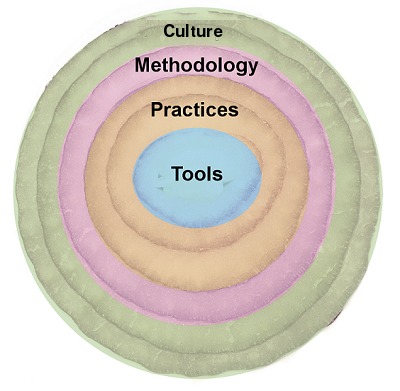
\includegraphics[width=0.5\linewidth]{onion}
            \caption{The full onion \cite{DaveSayers2013}}
            \label{fig:onion}
        \end{wrapfigure}
        As it was stated by Paul Hammon and John Allspawn at their \textit{10+ Deploys Per Day: Dev and Ops Cooperation at Flickr} presentation, tools and processes alone are not enough and the cultural change should be the first step to take towards DevOps. \\
        Because of this, the outermost represents the most important layer and without \textit{peeling} it you will not be able to access the inner layers.

        \subsection{A DevOps definition} \label{chap:stateoftheart:sec:devops:sec:definition}
        DevOps vastness can be seen in the enormous ammounts of tools categories identified in \ref{chap:stateoftheart:sec:devops:sec:tools} related with DevOps.\\
        As one might expect from this vastness of areas that DevOps touches, there are still difficulties to properly define DevOps. In order to reduce this indefinition, we will use throughout this thesis a conjugation of two definitions for DevOps.\\
        The first definition is from \textit{DevOps: A Software Architect's Perspective} \cite{Bass} and it states that: \\
        \textit{DevOps is a set of practices intended to reduce the time between committing a change to a system and the change being placed into normal production, while ensuring high quality.} \\
        We chose this definition because it allows to easily classify something as being DevOps or not i.e. one would only have to ask himself if a practice or cultural aspect will allow for the reduction of time since commiting a change until that change is in production, if it does, then it is DevOps. Nevertheless, we find this definition to be a bit empty in the sense that by only reading it one would not be aware of the aspects that are associated with Devops. As a workaround for this problem we use a second definition based on the CAMS acronym.\\
        The CAMS acronym \cite{Willis2010} defines DevOps as being a \textbf{C}ultural movement where \textbf{A}utomation and continuous \textbf{M}easurement of processes and people are promoted and where the later can serve as a input for the \textbf{S}haring of problems and new ideas. As new ideas appear to solve the indentified problems, new measurements can be made to further identify problems furthering improving the overall process.

        \subsection{DevOps Benefits}
        In a recent study \cite{Elliot2015} some of the DevOps benefits were identified:
  		  \begin{itemize}
  			    \item DevOps projects are believed to accelerate in 15\%-20\% the ability to delivery of capabilities to the client
            \item Adopting DevOps allows business to practice Continuous Delivery.
            \item The average cost of a critical application failure per hour is \$500,000 to \$1 million (DevOps can help reduce application failures).
            \item The average cost percentage (per year) of a single application's development, testing, deployment, and operations life cycle considered wasteful and unnecessary is 25\% (DevOps can help automate some repetitive tasks)
  		  \end{itemize}

      \subsection{Patterns}
      Some previous progress has already been made regarding the identification of DevOps related patterns. We will summarize this progress by listing the identified patterns and briefly describing them:
      \begin{itemize}
        \item \textbf{Store Big Files in Cloud Storages}\cite{Cukier2013} - Instead of creating and managing a system to store large files, or storing them in database columns, store them in a Cloud Storage\footnote{A storage system provided by a cloud provider.}
        \item \textbf{Queue based solution to process asynchronous jobs}\cite{Cukier2013} - When there are tasks that take a long time to complete but users still expect a quick response, create a new Job instance in a queueing service and then have a service performing those tasks. When finished, post the result of that Job somewhere acessible to the user and notify the user that the task is done.
        \item \textbf{Prefer PaaS over IaaS}\cite{Cukier2013} - For non technology companies, PaaS is usually preferable because it will give them lot of functionalities without the need for configuration. This will allow them to simply focus on their core business.
        \item \textbf{Load Balancing Application Server with memcached user sessions}\cite{Cukier2013} - Use a load balancer in front of your application servers. This severs will handle sessions using memcached which means that if a application server goes down or if a new application server is needed, it will be able to use the user session.
        \item \textbf{Email delivery}\cite{Cukier2013} - Rather than implementing your own SMTP solution, use cloud mail delivery services which provicde REST API's to send emails.
        \item \textbf{Logging}\cite{Cukier2013} - Having multiple servers you need a way to consolidate your application logs. In order to do so, you should use a cloud based log service.
        \item \textbf{Realtime User Monitoring (RUM)}\cite{Cukier2013} - Monitor user behaviour in order to find possible bugs or errors.
        \item \textbf{The isolation by containerization pattern} \cite{Sousa2015} - \say{Use a container to package the applications and its dependencies and deploy the service within it}.
        \item \textbf{The discovery by local reverse proxy pattern} \cite{Sousa2015} - \say{Configure a service port for each service, which is routed locally from each server to the proper destination using a reverse proxy.}
        \item \textbf{The orchestration by resource offering pattern} \cite{Sousa2015} - \say{Orchestrate services in a cluster based on each host’s resource-offering announcements.}

      \end{itemize}


  	\section{The Portuguese startup scene} \label{sec:stateoftheart:sec:portuguesestartupscene}
    Motivated by a recent investment in innovation and entrepreneurship, Portugal startups have been growing their position in the global startup scene \cite{Coleman2015}.

    A study from 2015 \citet{StartupEuropePartnership2015} in which the Portuguese startup scene was analyzed, revealed that there were already 40 technology scaleups \footnote{Scaleups are companies that raised more than \$1M funding (since foundation) and had at least one funding event in the last five-year period } operating in Portugal at the time. The same study stated that this startups were able to raise a large portion of the received investment from international investors indicating, therefore, that the reach and scale of this startups was broader than just the national arena. Additionally, it is also indicated in the study that Porto and Lisbon are the main centers of innovation, encompassing 70\% of the total of existing scaleups. In addition to the scaleups identified other smaller scale startups exist. Some of this startups are currently being incubated in incubators around the country. UPTEC \footnote{Science and Technology Park of University of Porto} and Startup Lisboa, both business incubators. This incubators had, at the time of this study more than 300 companies \cite{Uptec,StartupLisboa} under their wing.


    \section{A pattern language}
    Pattern languages have been used in the software development area in the past for describing common architectural solutions \cite{kircher2013pattern}, recurring software design choices \cite{johnson1995design} and even describing pattern languages themselves \cite{Meszaros1998}.\\
    Patterns represent a way to share recurring solutions to a problem \cite{Meszaros1998}. As a result, pattern languages help reduce re-discovery and re-invention of concepts and functionalities as well as \textit{avoiding common pitfalls that are learned from experience} \cite{Schmidt1995}.

\chapter{Towards DevOps} \label{chap:towardsdevops}
    In this chapter we will look at the approach used in order to solve the problem described in \ref{chap:introduction:sec:problem}. We will start by looking at how we defined the sample from which we extracted information and then how we handle that data in order to produce the final results.

    \section{Methodology} \label{chap:towardsdevops:sec:methodology}
      In \ref{chap:stateoftheart:sec:devops} we saw that the DevOps movement emerged in the software development\footnote{software development should be seen in this context as both the development, maintenance and any other tasks related with the creation of software} community. Having this factor into consideration and knowing that there is still a significant lack of scientific information regarding the subject, we choose to look for a solution within the development community. We believed, before conducting this study, that not only would they be able to provide us that information, but because they were using this techniques/tools in their daily activities, it would serve also an extra layer of assurance.

      \subsection{Adjusting Granularity}
        The vast number of existing tool categories \label{chap:stateoftheart:sec:devops:sec:tools} as well as the fact that there are a lot of possible practices that can be considered part of DevOps \ref{chap:stateoftheart:sec:devops:sec:definition} means that fully capturing the ideals and ideas related with it would not only be a tremendously hard task but would also not fit in the length of this thesis. \\
        Taking this into consideration and in order to avoid over specializing this thesis in some particular area, we set the desired granularity for the study by defining that we would only focus on categories of practices and if needed tools e.g. we wanted to know what steps did the Continuous Integration server run, but we were not interested in fully documenting the tool or measuring the time it took to run a full integration cycle. \\



      \subsection{Collecting the information}
      Taking into consideration the vastness of topics that DevOps \ref{chap:stateoftheart:sec:devops:sec:definition} touches, we knew that it would be hard to create a form that covered that extensively.\\
      It was theorized, at this point, that not all startups would have similar levels of maturity(we later observed this to be true \ref{anexes:interviews}). This meant that even if we could create this form, it would be too extensive for some cases and we would still have to create an all englobing form to capture all the information. \\
      The chosen methodoly adopted was to do a more exploratory type of interview. This idea lead to the creation of a script rather than a form that would guide the interviews. This script \ref{anexes:interview} had 5 major sections:
      \begin{itemize}
          \item \textbf{Product} - The product section would try to understand, first what did the company do and secondly if there were any kind of special requirements that would influence the choices made by the company.
          \item \textbf{Team Management} - Team sizes, interactions, project management techniques would be analyzed here.
          \item \textbf{Software delivery pipeline} - In this section, we identified if teams did Continuous Integration, how did they handled the creation of environments for each of the pipeline states and what teams did what in each state.
          \item \textbf{Infrastructure Management} - We tried to capture how the companies handled their infrastructer. Did they use the cloud? Which processes did they automate?
          \item \textbf{Monitoring \& Error Handling} - With this section we aimed to understand if the companies were monitoring their infrastructure, how did they do it and, when errors were detected, how were they responding?
      \end{itemize}

      \subsection{Defining a sample} \label{chap:towardsdevops:sec:methodology:sec:sample}
      As it was seen in \ref{sec:stateoftheart:sec:portuguesestartupscene}, Portugal has a rich startup community.\\
       Startups have strict contraints regarding the ammount of resources they have at their disposal and have, as a result, aditional incentive to automate as many tasks as they can. \\
      Being small (in terms of staff), communication and cultural aspects are usually guided towards cooperation as this is a key factor in allowing small teams to handle large projects. \\
      Finally, the fact that startups have as their objective to scale, further highlighs the need for automation and cooperation.\\
      This conjugation of factors meant that the mindset of startups was aligned with the DevOps one and startups are therefore a good place to look for information that can be directly linked to DevOps.\\
      Having more than 300 startup companies \ref{sec:stateoftheart:sec:portuguesestartupscene} from which to choose, we needed a way to filter out companies that may not be relevant to our study. \\
      With that objective we first created a list of all the startups companies we knew that operated in Portugal. This list was create by looking at some of the Portuguese startup incubators and by extracting the list of companies. \\
      From those 300 startups, we attempted to identify which ones were doing software development. To do so we looked, when available, at the company web page and tried to determine if the company product was software related or not. This approach reduced the number of companies to 155.

      Then, we prioritize which companies were better or worst for our study. To do so we created a compound evaluation metric that would allow us to rank companies. We created 5 metrics to do so:
      \begin{itemize}
        \item \textbf{Cloud Usage} - We created three possible values for this metric. If a company used cloud services, we would give the company 2 points. If we were not sure if a company was using cloud services, we would give it 1 point. If we know the company was not using cloud services, we would give it 0 points. With this metric we attempted to distinguish between, for instance, companies that were developing hardware solutions from those that were developing more software oriented solutions.

        \item \textbf{SaaS/PaaS offering} - Having the same point attribution schema as the \textit{Cloud Usage} metric we believed that if a company had a SaaS/PaaS product, it would need to have some sort of automation put into practice as it would need to be able to scale if there was a sudden increase in clients.

        \item \textbf{Company Size} - We create four possible values for each metric. Companies could have 0,1,2,3 points if they had respectively less than 5 members, between 5 and 15 memebrs, more than fifteen members or more than fifteen members and several teams.

        \item \textbf{Subjective Appreciation} - This metric would reflect the overall opinion of the company that we developed when searching for information for the other metrics. Some common factors that influenced this metric were for instance the fact that some companies had listed staff members working on software development task, or if the company website was down.
      \end{itemize}

      The resulting ranking, created by summing all the factors, is not supposed to be seen as a precise way to accurately compare companies i.e. the second company maybe as relevant as the first one, but rather as a way to prioritize them, i.e. the first company surely is more intersting to study then the last one.

      In the end, we contacted a total of 60 companies from which we were able to interview 25.

      \subsection{Sample Characterization}
      The sample, as seen in fig. \ref{fig:companymembers} was mostly composed of small companies with no more than 35 employees and with half of the sample size to have less than 15 members. The companies also conducted a substancial amount of their business over the internet either through a browser application or a mobile app or a combination of both.
      \begin{figure}
        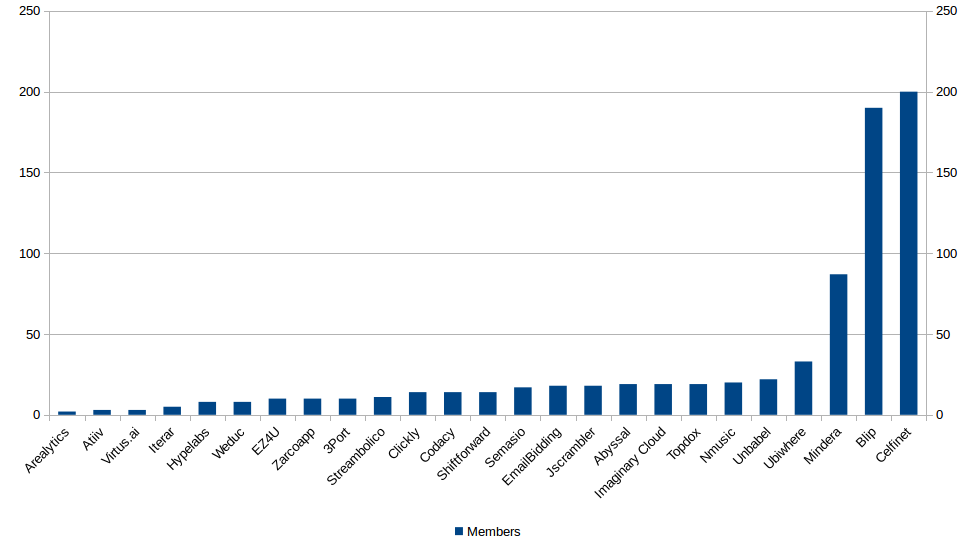
\includegraphics[width=1\linewidth]{companymembers}
        \caption{Studied companies size}
        \label{fig:companymembers}
      \end{figure}

      \subsection{Data Processing \& Pattern Extraction}
      After conducting the interviews, the next task was to analyze and process the collected information.\\
      Fig. \ref{fig:concepts} shows how we merged some of the identified techniques into larger groups that would represent patterns. The full grouping can be found in \ref{anex:pat:group}.\\
      \begin{figure}
        \centering
        \includegraphics[width=0.4\linewidth]{concepts_partial}
        \caption{Identified concepts and subsequent refining}
        \label{fig:concepts}
      \end{figure}
      As this was being done, it became clear that, because of the size of the sample (25 companies), this study would not be statistically significant. Nevetheless we found that the information we gathered had value and would be able to provide future studies with usefull pointers on how to approach the problem.\\
       Due to the fact that some practices were rare, we had to group them into categories in order to have a representative value inside the sample, e.g. some companies would run integration tests on their CI tool while others would only run unitary tests; both would, nevertheless, run tests. \\
      Using this groupings, we were able to identify a set of problems that companies were solving using different approaches. We were able, as a result, to extract in total 13 patterns each representing a problem and providing a set of solutions that took into consideration the context of the company. The final list of practices and frequencies can be found in \ref{anex:pat:freq}.
      This set of patterns can be found in chapter \ref{chap:patterns}

     \subsection{Patterns}
      Throughout the interviews we noted several tendencies. \\
      The first was the widespread use of Cloud computing with 76\% of the interviewed companies using it. Then there was the dominance of Git as the version control system with 80\% of the interviewees using it as their version control system. Chat and direct communication were also the main ways chose by companies to communicate (100\%). \\
      Being able to measure some of the key business metrics like the health of the system is also a concern for most companies with almost 70\% of them having some sort of system to do so. \\
      Having a way to replicate environments was also a major trend among companies with 60\% of companies already adopting one way to do so. \\
      The following table(tab. \ref{table:categories}) enumerates the categories of problems identified with the percentage of interviewed companies that were handling that problem. These problems will be further developed in chapter \ref{chap:patterns}

      \begin{table}[h!]
        \begin{center}
            \begin{tabular}{| p{0.5\linewidth} | p{0.5\linewidth} |}
            \hline
            \textbf{Categories} & \textbf{\% of companies that solved the problem} \\ \hline
                  Version Control                       & 100\% \\ \hline
                  Communication                         & 100\% \\ \hline
                  Cloud                                 & 84\%  \\ \hline
                  Auditability                          & 68\%  \\ \hline
                  Continuous Integration                & 64\%  \\ \hline
                  Error Handling                        & 60\%  \\ \hline
                  Reproducible Environments             & 60\%  \\ \hline
                  Scalling                              & 48\%  \\ \hline
                  Code Review                           & 44\%  \\ \hline
                  New Computing Instances Deployment    & 44\%  \\ \hline
                  Error Alerting                        & 36\%  \\ \hline
                  Job Scheduling                        & 12\%  \\ \hline
            \end{tabular}
        \end{center}
        \caption{Categories frequency}
        \label{table:categories}
      \end{table}
% \begin{pattern}{}
% 	\context{}
% 	\problem{}
% 	\solution{}
% \end{pattern}
\chapter{ Patterns } \label{chap:patterns}
	% \section {Architecture} \label{chap:patterns:sec:architecture}

	% 	\begin{pattern}{Microservices} \label{chap:patterns:sec:architecture:p:microservices}
			
	% 		\context{A complex application is developed and maintained by several people.}
			
	% 		\problem{Maintaining a big and complex application is difficult.}
			
	% 		\solution{Break the application into several services that communicate with each other.}
	% 	\end{pattern}


	\section{Acquiring Computing Resources} \label{chap:patterns:sec:acquiringresources}
		Entities usually have the need to have a \textbf{web} presence or to acquire computing resources to do some tipe of processing. This means that computing resources must be acquired. 
		
		\begin{pattern}{Cloud} \label{chap:patterns:sec:acquiringresources:upinthecloud}
			\context{You have a piece of software that you want to make available for people to interact with. 

			Because of its size, complexity, distributed nature, etc, you do not want people to have to install that piece of software on their devices. 

			In order to allow people to interact with your software you have therefore to have some underlying infrastructure to support your needs. 

			}
			\problem{How do setup/acquire infrastructure/resources in order to meet your needs ?}
			
			\forces{
				\begin{itemize}
					\item Hardware is expensive to buy and you may only need it for a short period.
					\item Hiring a team/person for managing and maintaining your hardware is expensive. 
					\item In the future resource needs may vary and you may want to increase or decrease your computational resources.
				\end{itemize}
			}
			\solution{Cloud providers allow individuals and businesses to purchase computing resources with a \textbf{pay-as-you-go} business model. Cloud providers assume the responsabilitie of \textbf{maintaining} and \textbf{managing} the physical infrastructure.}
			\rationale{Due to its scale cloud providers can usually provide a competitive price compared to the price of maintaing you own infrastructure. The pay-as-you-go model allows you to allocate and deallocate resources meaning that you are only using what you need. Together with the fact that no hardware upfront costs are required this means that using the cloud is usually the best alternative.}
		\end{pattern}

		\begin{pattern}{Platform as a Service}
			\context{You have decided to use the \textit{Cloud}.

			The software you want to deploy follows common flows of installation/setup and you do not need a lot of access to the underlying infrastructure.

			}
			\problem{Cloud providers offer a set of different types of services and you do not know which to use ?}
			\forces{
				\begin{itemize}
					\item Platform as a Service usually allow for some configuration of the underlying layer.
					\item Platform as a Service environments are usually managed by the provider.
					\item Platform as a Service is usually expensier than Infrastructure as a Service.
				\end{itemize}

			}
			\solution{Deploy your software by using a Platform as a Service.}
			\rationale{PaaS pushes the environment management to the provider. This means that you do not have to alocate people and time to manage it. This does not mean however that there is no control, some configuration can still be specified by the user.}
		\end{pattern}

		\begin{pattern}{Infrastructure as a Service}
			\context{You have decided to use the \textit{Cloud} and your application needs \textbf{very specif configurations} to be deployed or you need access to the undelying infrastructure.}
			\problem{What aaS model should you use?}
			\forces{
				\begin{itemize}
					\item Using Infrastructure as a Service means having the responsability of configuring and maintainig all machines.
					\item Pricewise Infrastructure as a Service is usually the cheapest of the aaS.
				\end{itemize}
			}
			\solution{Deploy your software by using IaaS}
			\rationale{IaaS gives fine grain control over the aspects of the infrastructure. Cloud providers allow for the allocation of virtual machines that are fully configurable.}
		\end{pattern}








	\section {Reproducible Environments}
		
		\begin{pattern}{Containers}
			\context{You have or want to have several instances of your software installed in several machines. Your instances may need to be updated/altered both in terms of the software they run but also the environment on wich it runs. }
			\problem{How do you make sure that the environments were your code run are consistent across all machines even when changes are applied ?}
			\forces{
				\begin{itemize}
					\item Performing manual installations can lead to errors.
					\item Manually installing or updating dependencies and configuring machines is time consuming.
					\item If changes are costly there will be an incentive not perform them.
				\end{itemize}
			}
			\solution{Containerize your applications by creating a container that includes among other things all of your dependencies and configurations.}
		\end{pattern}

		\begin{pattern}{Virtual Machine}
			\context{You have or want to have several instances of your software installed in several machines. Your instances may need to be updated/altered both in terms of the software they run but also the environment on wich it runs.}
			\problem{How do you make sure that the environments were your code run are consistent across all machines and that changes to that environment can be easily applied ?}
			\forces{
				\begin{itemize}
					\item Performing manual installations can lead to errors.
					\item Manually installing or updating dependencies and configuring machines is time consuming.
					\item If changes are costly there will be an incentive not perform them.
				\end{itemize}
			}
			\solution{Create a \textbf{image} of the machine desired.\newline That machine image can then be copied and used to setup a reproducible environment.}
		\end{pattern}

		\begin{pattern}{Scripting}
			\context{ou have or want to have several instances of your software installed in several machines. Your instances may need to be updated/altered both in terms of the software they run but also the environment on wich it runs.}
			\problem{How do you make sure that the environments were your code run are consistent across all machines and that changes to that environment can be easily applied ?}
			\forces{
				\begin{itemize}
					\item Performing manual installations can lead to errors.
					\item Manually installing or updating dependencies and configuring machines is time consuming.
					\item If changes are costly there will be an incentive not perform them.
				\end{itemize}
			}
			\solution{Create a script that describes your infrastructure dependencies and configurations. This script can then be used in several machines to create similar environments.}
		\end{pattern}

	\section{Creating a new instance}
		\begin{pattern}{Download the Virtual Machine image}
			\context{You have choose to define your infrastructure using a \textit{Virtual Machine} and you want to create a new runnning instance of your software. }
			\problem{How do you do it ?}
			\forces{
				\begin{itemize}
					\item Rebuilding the image takes time and depending on how you setup the image build the final image may be different across builds.
					\item Some of your dependencies may need to be downloaded from external providers. If they fail usually your build fails.
				\end{itemize}
			}
			\solution{Build the image you want to run once. Then make it available for download and reuse it.}
		\end{pattern}

		\begin{pattern}{Pull the container}
			\context{You have choose to define your infrastructure using a \textit{Containers} and you want to create a new runnning instance of your software. }
			\problem{How do you do it ?}
			\forces{
				\begin{itemize}
					\item Rebuilding a container takes time and depending on how you setup the container build the final container may be different across builds.
					\item Some of your dependencies may need to be downloaded from external providers. If they fail usually your build fails.
					\item If the environment setup has some complex or time-consuming steps you may take a long time to build single a container.
				\end{itemize}
			}
			\solution{Build the container once. Then make it available for download and reuse it.}
		\end{pattern}

		\begin{pattern}{Anti: Run the script}
			\context{You have choose to define your infrastructure using only \textit{Scripts} and you want to create a new runnning instance of your software. }
			\problem{How do you do it ?}
			\forces{
				\begin{itemize}
					\item Some of your dependencies may need to be downloaded from external providers. If they fail usually your script fails.
					\item Re running the script takes time and depending on how you setup the script inconsistencies can arise.
				\end{itemize}
			}
			\solution{Run the script that does the configuration of the application environment in the machine were you want to install the application.}
		\end{pattern}

	\section{Scalling Infrastructure}
		\begin{pattern}{Anti: Vertical Scalling}
			\context{You have variable usage of your infrastructural resources. You may need to quicly increase or decrease the size of the infrastructure to meet your needs.}
			\problem{How do you scale your computing capacity in order to respond to the change.}
			\forces{
				\begin{itemize}
					\item Due to physical constraints there is a limit for how many resources you can alocate to a single machine.
					\item Increasing the resources of one machine may not increase the throughput of the overall system.
					\item There are no special considerations to have when designing a system in order for it to scale vertically. 
				\end{itemize}
			}
			\solution{You can increase your computing resources by adding memory to your machine or by increasing the number of cores your machine has.}
		\end{pattern}
		\begin{pattern}{Horizontal Scalling}
			\context{You have variable usage of your infrastructural resources. You may need to quicly increase or decrease the size of the infrastructure to meet your needs.}
			\problem{How do you scale your computing capacity in order to respond to the change.}
			\forces{
				\begin{itemize}
					\item If you are using the \textit{Cloud} you have virtually no limit to how many machines you can allocate.
					\item Horizontally scalable systems are more challenging.
					\item Having several machines allows you to have some redundancy making your system more robust.
					\item Having more machines 
				\end{itemize}
			}
			\solution{You alocate new machines to your project.}
		\end{pattern}

	\section{Testing}

		\begin{pattern}{Anti: Manual Testing}
			\context{You are building a software product and are constantly improving it. }
			\problem{Whenever you make a change how will you know that the software still works.}
			\forces{
				\begin{itemize}
				\item Changes to even a small functionality may have impact on a completely unrelated functionality of the system.
					\item Deploying new features without testing the entire system may result in failure.
					\item Manually testing all aspects of your application may take a long time.
				\end{itemize}
			}
			\solution{You charge your developer with the responsability of making sure that the software is functional after he made the changes. The developer usually develops the changes to the software and then procedes to manually test the system.}
		\end{pattern}

		\begin{pattern}{Automatic Testing}
			\context{You are building a software product and are constantly improving it.}
			\problem{Whenever you make a change how will you know that the software still works.}
			\forces{
				\begin{itemize}
					\item Changes to even a small functionality may have impact on a completely unrelated functionality of the system.
					\item Deploying new features without testing the entire system may result in failure.
					\item Manually testing all aspects of your application may take a long time.
					\item Developing automatic tests is additional work and may increase the time needed to develop a feature.
					\item Some functionalities of your software may not be testable. 
				\end{itemize}
			}
			\solution{You charge your team with the responsability of developing automated tests(unitary and/or integration and/or functional) for your software. The code is developed and with it the new tests that test that the new changes are working.}
		\end{pattern}

	\section{Continuous Integration}
		\begin{pattern}{Continuous Integration}
			\context{You have several people/teams contributing to the same codebase.}
			\problem{Whenever a change is made to your project you want to know that the change did not break anything.}
			\forces{
				\begin{itemize}
					\item Whenever something stops working you want to know when did it stop.
					\item Having quick feedback may help you figure out a solution faster because you still remember what you have done.
				\end{itemize}
			}
			\solution{You use an automatic system of \textit{Continuous Integration} that \textit{Build}s, \textit{Test}s the new version of the software and provides \textit{Feedback}.}
		\end{pattern}

		\begin{pattern}{Build}
			\context{Your have a change in your software and.}
			\problem{How do you construct new shipable version of your project ?}
			\solution{If you have a \textit{Container} and are able to \textit{Download the container} you can obtain the container with the new version of the software . The same can be done using \textit{Virtual Machine} and \textit{Download the Virtual Machine}}.
		\end{pattern}

		\begin{pattern}{Test}
			\problem{Whitin your \textit{Continuous Integration} you have successfully created and built the software.}
			\context{You want to know that the build you generated works.}
			\solution{Use the \textit{Automatic Testing} and run your entire suit of tests within the new build.}
		\end{pattern}

		\begin{pattern}{Notify}
			\problem{You have \textit{Build} and run all the \textit{Test}s in your \textit{Continuous Integration} system.}
			\context{You want to communicate the result of those steps to your team.}
			\solution{You can communicate the result of the integration by using a \textit{Chat Tool} or by sending an \textit{Email} to the developer/team.}
		\end{pattern}


	\section{Version Control}
		\begin{pattern}{Git Flow}
			\context{You are using Git or a similar version control software for your code.}
			\problem{You want to organize your version control flow in a way that you separate what is being develop from what has been developed and from the current release/production code.}
			\solution{You can choose to divide your project in 3 branches. The master branch will represent a release or the version that is currently in production. The develop branch will represent all of the current developed features. For each new functionality a new branch will be created. Once terminated the feature if accepted (through pull request) will be merged into the develop branch. When you want to signal a new release you just merge the desired state of the develop branch into the master branch. }
		\end{pattern}
		\begin{pattern}{Feature Branches}
			\context{You are using Git or a similar version control software for your code.}
			\problem{You want to organize your version control flow so that you separate what has been done from what is still being done.}
			\solution{You have a master branch. For each new feature you create a new branch. Once the feature is done you merge it into the master branch.}
		\end{pattern}
	\section{Teams}
		
		\begin{pattern}{Anti: Specialized Teams}
			\context{You have a set of professionals that you want to allocate to one or several projects.}
			\problem{You want to organize them in a productive way.}
			\solution{You divide them by specializations and have them work separately.}
		\end{pattern}

		\begin{pattern}{Multidisciplinary}
			\context{You have a set of professionals that you want to allocate to one or several projects.}
			\problem{You want to organize them in a efficient way that allows them to quicly adapt to new problems.}
			\solution{You create teams that include individuals from different disciplines.}
		\end{pattern}

		\begin{pattern}{Keep it Small}
			\context{}
			\problem{You do not know how many people to allocate to the project team.}
			\solution{Depending on your needs you could allocate between 1 and 9 people.}
		\end{pattern}

		\begin{pattern}{Keep it loose}
			\context{}
			\problem{You do not know how to hierarchical organize people to the project.}
			\solution{You create an horizontal structure inside your team and let them organize themselves.}
		\end{pattern}

	\section{Communication}
		\begin{pattern}{The direct communicator}
			\context{People with different backgrounds and degrees of knowledge are working together.}
			\problem{You want knowledge and ideas to be shared between people.}
			\solution{Allow you team members to communicate directly.}
		\end{pattern}
		
		\begin{pattern}{Chat is for links files and winks}
			\context{Several people are working in the same project.}
			\problem{People want to share links and files.}
			\solution{Most chat tools allow for the sharing of files and links between members.}		
		\end{pattern}

		
	\section{Jobs}

		\begin{pattern}{Anti: Daemon}
			(Confirmar com EZ4U)
			\context{Your application has some maintenance or some backgrounds tasks that take a significant ammount of time to complete.}
			\problem{How do you do it?}
			\solution{You create a Daemon that sequencially performs each tasks and notifies some service or updates a service when the task is completed.}
		\end{pattern}

		\begin{pattern}{Launch new infrastructure}
			\problem{Your application has some maintenance or some backgrounds tasks that take a significant ammount of time to complete.}
			\solution{You sequencially launch a new piece of infrastructure to perform the task you have to perform.}
		\end{pattern}

	\section{Monitoring}
		\begin{pattern}{Monitor the present}
			\context{You have several servers.}
			\problem{You want to know wich ones are on and which ones are not.}
			\solution{You deploy a tool in each infrastrucuture element that tells a master one if that server is online or not.}
		\end{pattern}

		\begin{pattern}{Save the past}
			\context{You have several servers.}
			\problem{You want to know when there is a problem, what has happened.}
			\solution{You deploy a tool in each infrastrucuture element that reports to the master one the logs from your applications.}
		\end{pattern}

	\section{Alert}
		\begin{pattern}{Thresholding}
			\context{You have a need to watch over your infrastructure and you want to fix problems when they appear.}
			\problem{You do not want to have to have someone continuously looking to find possible problems.}
			\solution{Define indicators that try to assess your infrastructure . Define thresholds and alert levels for each indicator. When a treshold is exceeded an alert should be triggered. }
		\end{pattern}

		\begin{pattern}{Anti: Wake the devs}
			\context{You have defined tresholds and alert levels for your infrastructure.}
			\problem{You don't know who to contact.}
			\solution{You send an alert to everyone involved in the project.}
		\end{pattern}

		\begin{pattern}{Rotate and Wake}
			\context{You have defined tresholds and alert levels for your infrastructure.}
			\problem{You don't know who to contact.}
			\solution{You have an on call engineer and you rotate the position through the team. The notification is sent to that engineer.}
		\end{pattern}

	\section{Error Handling}

		\begin{pattern}{Rolling Back}
			\context{You have detected a problem in your production application.}
			\problem{You want to solve that problem.}
			\solution{You change the production version of your application to previously working version.}
		\end{pattern}

		\begin{pattern}{Rolling Back: DNS Switching}
			\context{You have detected a problem in your production application.}
			\problem{How do you change the live version to the previous one ?.}
			\solution{You change the DNS for it to point to the old version of the application.}
		\end{pattern}

		\begin{pattern}{Rolling Back: Deploy again}
			\context{You have detected a problem in your production application.}
			\problem{You want to solve that problem with minimu.}
			\solution{You do a normal deploy but choose the previous version.}
		\end{pattern}

		\begin{pattern}{Hotfix}
			\context{You have detected a problem in your production application.}
			\problem{You want to solve that problem with minimu.}
			\solution{You make the changes necessary to correct your application and then deploy this new version.}
		\end{pattern}


		\begin{figure}[p]
    		\makebox[\linewidth]{
        	\includegraphics[width=0.6\linewidth]
        	{./figures/map.png}
    	}
    	\caption{Pattern Map}
		\end{figure}



\chapter{ Validation } \label{chap:validation}


Validating the collected data and the subsequently identified patterns cannot be made in a formal way.

The only course of action available is therefore to measure the effects that applying the gathered information has in a real world situation. In order to do so, measurements must be made before and after the application.

\section{Criteria}

Having a wide are of application and focusing its attention in several areas and domains, measuring the success of adopting DevOps can be difficult. In this work the evaluation of the success factor will be divided into two main categories having each a set of criteria for acceptance:


	\begin{itemize}
        \item{ Technical aspects }
        	\begin{itemize}
				\item{Deployment Frequency} - Deploying an application is the process by which software can be made available to the customer. By increasing the deployment frequency teams can more frequently transmit value to the customer. 
                
				\item{Deployment Time} - Deployment time is of great importance as it enables companies to quickly respond to change. 
                
				\item{Infrastructure Elasticity} - Being able to quickly and in an automated way increase or decrease the infrastructure size can mean the difference between success and failure. 
                
			\end{itemize}
            
            
        \item{ Organizational aspects }
        	\begin{itemize}
				\item{Team satisfaction} - Team satisfaction is essential as it promotes more motivated professionals and better results.
                
				\item{ Managerial satisfaction } - The satisfaction of the managerial team is of great importance as it usually reflects the current state of the business. 
                
			\end{itemize}

	\end{itemize}


	For the previous criteria the following acceptance and rejection metrics will be used: 
    
		\begin{table}[h!]
			\centering
            \caption{Technological Criteria}
			\label{tab1}
			\begin{tabular}{|l|c|c|}
               	\hline
 				Criteria & Acceptance & Rejection  \\ \hline
 				Deployment Frequency & Increase  & Decrease   \\ \hline
 				Deployment Time & Decrease &  Increase  \\ \hline
 				Infrastructure Elasticity & Decrease & Increase \\ \hline 
			\end{tabular}
		\end{table}



		\begin{table}[h!]
			\centering
            \caption{Organizational Criteria}
			\label{tab2}
				\begin{tabular}{|l|c|c|}
                	\hline
 					Criteria & Acceptance & Rejection  \\ \hline
 					Team satisfaction & Increase  & Decrease   \\ \hline
 					Managerial Satisfaction & Increase &  Decrease  \\ \hline
 					Infrastructure Elasticity ( time to provision new resources) & Decrease & Increase \\ \hline 
				\end{tabular}
			\end{table}

	
\chapter{ Conclusions } \label{chap:conclusion}
    \section{Contributions}
    As of this moment, DevOps is still evolving and as more people join the discussion more perspectives and experiences will become part of the movement. Regardless, we believe that the initial work made in this thesis towards a more structured way of presenting and talking about DevOps will help reduce the barriers for new adopters and help the movement grow by providing a common dialect for discussing DevOps. This work can also be seen as a starting point for further investigation.



    \section{Future Work}
      \subsection{Specializing the identified patterns}
      While pursuing the study of DevOps we kept a high level of granularity with the objective of capturing a wider view of the movement and its practices. We believe that based on this work, each pattern can be further analyzed in a more precise way.
      \subsection{DevOps monitoring}
      As referred before, the DevOps movement is still evolving. We believed that, by monitoring the DevOps movement it will be possible to identify more practices being employed by companies and individuals.
      \subsection{Further validation}
      The initial results observed hint that DevOps and its practices can bring benefits to both companies and individuals. In this thesis we were not able to fully validate all of the identified patterns and we also did not observe long term effects of this developments in both teams and companies. Validation was also done with only one team and one company, which is insufficient to prove that those benefits can be reproduced in other teams or organizations.
      \subsection{Statistical Analysis}
      A statistical analysis of the practices and methodologies employed by startup companies should also be developed in order to validate if the presented patterns are indeed a common practice among them.

\bibliographystyle{abbrv} % or try abbrvnat or unsrtnat
\bibliography{references} % refers to example.bib

\appendix
\pagebreak
  \chapter{Annexes}
  \pagebreak

  \section{Pattern Map} \label{anex:pat:map}
    \begin{figure}[ht!]
        \includegraphics[width=1\linewidth]{./figures/patterns.png}
    \end{figure}
\pagebreak
  \section{Concepts Grouping} \label{anex:pat:group}
    \begin{figure}[ht!]
        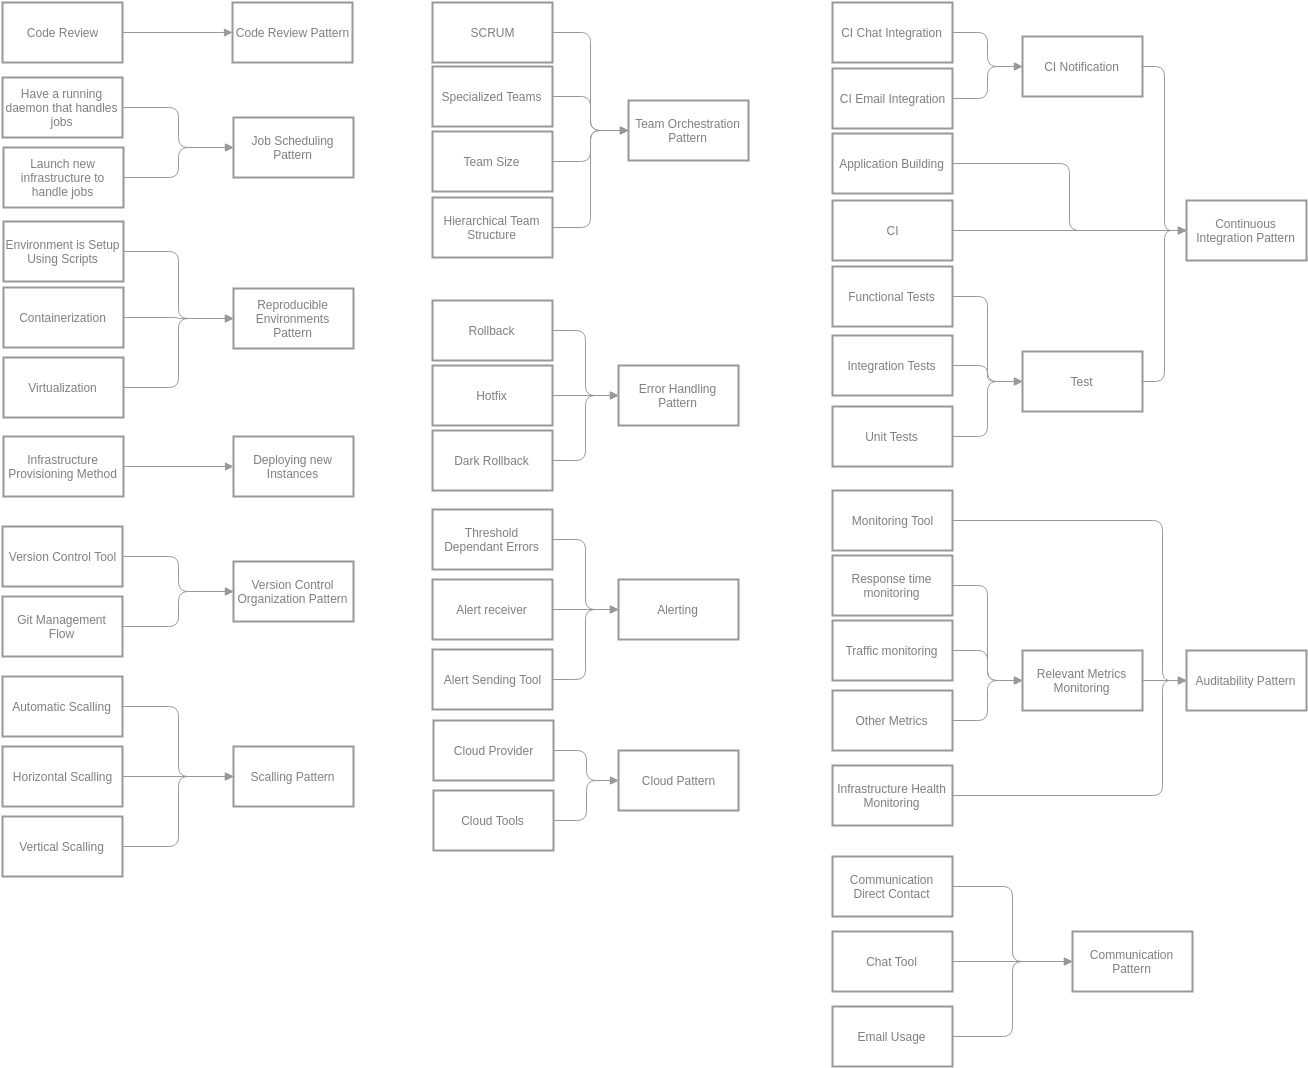
\includegraphics[width=1\linewidth]{./figures/concepts.png}
    \end{figure}
\pagebreak
\begin{landscape}
    \begin{figure}[ht!]
      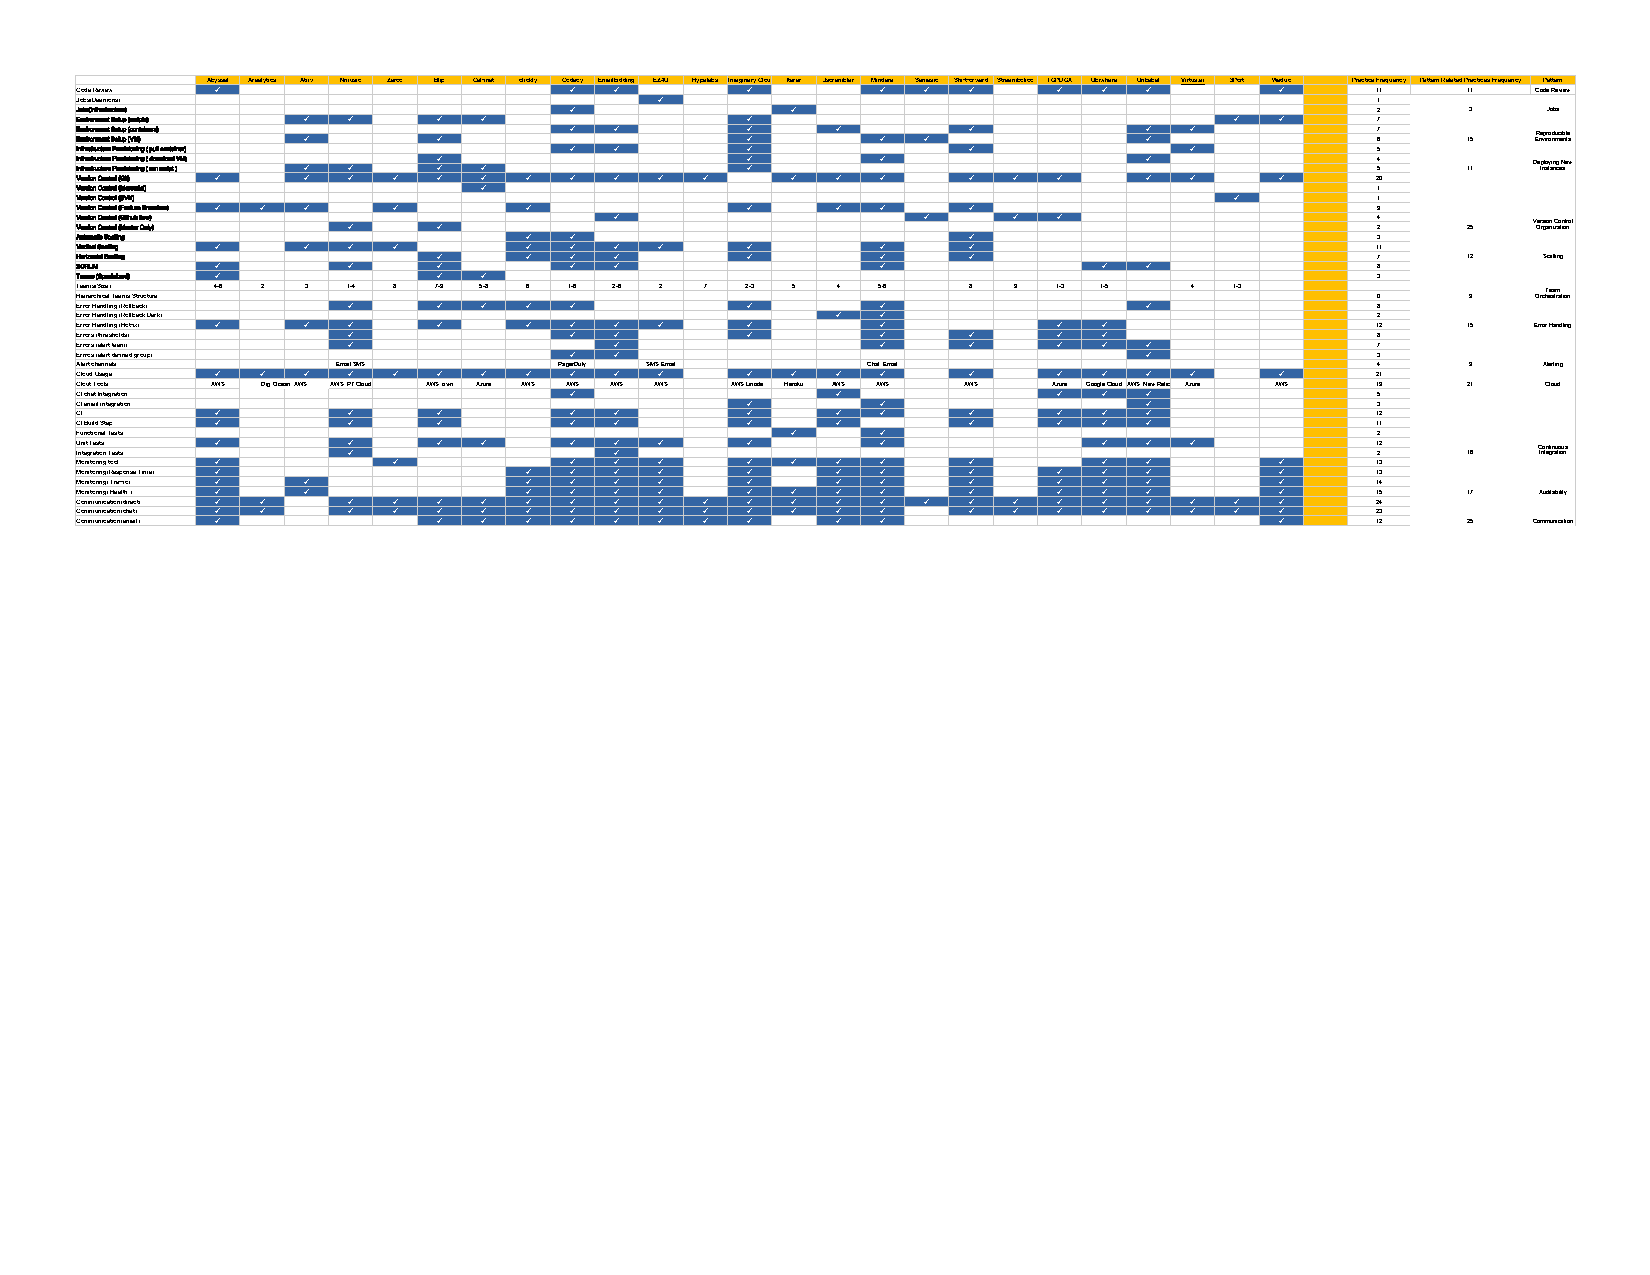
\includegraphics[height=0.8\linewidth]{patterns_stats.pdf}
      \caption{Interview practices frequency extraction.}
      \label{anex:pat:freq}
    \end{figure}
\end{landscape}

\pagebreak

  \section{Interview Guide} \label{anexes:interview}
    \subsection*{Product}
        \begin{itemize}
            \item What type of product do you develop ?
            \item What is the scale of that product ? Number of countries, number of users ?
            \item Do you have some kind of SLA or some requirements that impacts your work ?
    \end{itemize}
    \subsection*{Teams}
        \begin{itemize}
            \item How many teams do you have ?
            \item What is the size of each team ?
            \item Are teams specicalized or do they have multiple specializations working together ?
            \item Do teams interact with each other ?
            \item How are teams seen from an external perspective ? Are they autonomous?
            \item How do you manage your workload ? Do you use SCRUM,Kanban or other ?
            \item How do team members communicate among themselves.
    \end{itemize}
    \subsection*{Pipeline}
  	    \begin{itemize}
            \item How long does your code take to go from idea to production ?
            \item What are the states that you code goes through before reaching a production environment
            \item What triggers the transition between states ?
            \item What kind of tests do you develop? Which teams are involved in that process ? When do they run?
            \item What happens in each of the pipeline states ?
            \item In each state, which teams intervene and what do they do?
            \item What processes did you automate ? Did you choose to not automate some state ? If so, why?
            \item How do you handle your deployment process ? Which tools do you use ? Do you use containers or VMs ?
    \end{itemize}
    \subsection*{Infrastructure Management}
        \begin{itemize}
            \item How do you scale ? Horizontally or vertically?
            \item Does scalling happen automtatically ?
            \item What can make infrastructure scale up/down ?
            \item How is infrastructure increased ?
            \item How do you lift new instances of your infrastructure? Is it automatic?
    \end{itemize}
    \subsection*{Monitoring \& Error Handling}
  	    \begin{itemize}
            \item What metrics do you collect from running servers ?
            \item What do you see as errors ?
            \item What process do you follow to solve errors after they are detected ?
            \item When errors are detected, who is notified ? How is the notification sent ?
            \item If errors are detected before the software reaches production, what do you do ?
        \end{itemize}
\pagebreak

  \section{Companie Interviews Report} \label{anexes:interviews}
    \begin{companyreport}{Abyssal}
        \product
        Abyssal is a startup company focused on developing Subsea Navigation Systems for Remotely Operated Vehicles (ROVs) operating since 1 de Fevereiro 2012.\\
        Their goal is to facilitate the access to these locations by developing intuitive and precise software solutions to the major problems affecting ROV piloting and supervision: poor navigation, reduced visibility and lack of spatial\\ awareness.\\
        The current solutions has two major modules. One that renders the underwater obstacles in the live video feed from the ROVs and a web one that handles the transmission of data from the rig/ship to shore.
        \teams
        Teams at abyssal are mainly divided by area of specialization and have between 6-4 people. Nevertheless, roles inside each team sometimes change(see below). Teams communicate both directly and through Slack. Confluence is used as as a collaboration platform.\\
        In order to manage the project, Abyssal uses SCRUM.
        \development
        The development process at abyssal focus on three languages : C++. C\# and Python. In order to manage their code, Abyssal uses Git with feature branches.\\
        Unitary tests are developed by the development team, manual tests are performed by one member of the development team (the role is changed every sprint). This unitary tests are then used in the Continuous Integration phase.\\
        A code review process was also implemented. Every feature is analysed by one member of the development team. This member must not be the same one that did the feature.\\
        Continuous Integration is managed by Team City. Team City is responsible for creating a build and running the existent tests.
        \operations
        Abyssal uses AWS services in order to manage their infrastructure. Due to well defined upper and lower bounds for users numbers and load scaling is done only manually at Abyssal.\\
        Deployments and upgrades are mainly managed  manually except for the Virtual Reality where a tool assists the the deployment process.\\
        Logs are stored in the running instances and retrieved manually when needed.\\
        Monitoring relies on AWS services and the main metrics monitored are server load and and disk space.\\
        When errors are detected, Abyssal usually solves them by issuing a hotfix.
        \reportend
    \end{companyreport}

    \begin{companyreport}{arealytic}
      \product
      arealytic is a young company ( 5 month old in the time this interview was conducted) that wants to transform IP  and other types of cameras into analytics tools. In order to do this, arealytic developed a web platform that analyzes camera footage and tracks user movements throughout a store as well as interactions with displayed products.\\
      \teams
      The arealytic team had at the time two members. Both worked in all aspects of the product and communicated either directly or by using Slack.\\
      \development
      The development process at abyssal focus on three languages : PHP, Javascript and Python. In order to manage their code, arealytic uses Git with feature branches.\\
      \reportend
    \end{companyreport}

    \begin{companyreport}{Atiiv}
      \product
      Atiiv is a company that develops a web platform for Personal Trainers to monitor, register and prescribe training plans to it's clients.\\
      At the time of the interview the company was roughly 1.5 years old and had 4 collaborators.\\
      \teams
      Teams at Atiiv have 3 people and communicate  using several a chat tool.
      \development
      The development process at Atiiv focus on two languages: PHP and Javascritp . In order to manage their code, Atiiv uses Git  with feature branches. \\
      Unitary tests are developed by the development team, manual tests are also performed by the development team.
      \operations
      Atiiv uses Digital Ocean and AWS services in order to manage their infrastructure.  \\
      Deployments and upgrades are managed by Laravel Forge (a PaaS service). \\
      Monitoring relies on New Relic services and some of the metrics monitored are the server state and load. \\
      When errors are detected, Atiiv usually solves them by doing a hotfix.
      \reportend
    \end{companyreport}

    \begin{companyreport}{NMusic}
      \product
      NMusic is a portuguese startup that develops a platform that allows other businesses to stream and synchronize music.
      \teams
      Teams at NMusic are mainly divided by speciality and have between 1-4 people. Teams communicate  both directly for doubts and discussions and using Slack to share files and links.
      \development
      In order to manage their code, NMusic uses Git with only a master branch.  \\
      Unit tests are developed by the Development team and manual tests are performed by a QA team. \\
      Continuous Integration is managed by Jenkins and its main objective is to create a nightly build . This tool is  responsible for creating a build and running the existing tests.
      \operations
      NMusic uses AWS and PT Cloud services in order to manage their infrastructure.\\
      Deployments and upgrades managed by Capistrano .\\
      Monitoring relies on Zabbix. If errors are detected depending on their severity different approaches can be adopted. If an error is not critical, an internal interface will be updated, if an error is bad but still not critical, an email is sent. In a case where an error is considered critical there are two developers that are notified by SMS. Some common solutions at NMusic can be issuing a hotfix or deploying the previous version.
      \reportend
    \end{companyreport}

    \begin{companyreport}{Zarco}
      \product
      Zarco is a mobile app that aims to link travelers with traveling guides.
      \teams
      The Zarco team has 8 members. The team communicates directly{for doubts and discussions} or by using Slack(to share files and links).
      \development
      The development process at Zarco focus on Java, Javascript Swift  and PHP. In order to manage their code, Zarco uses Git with Feature Branches.
      \operations
      Zarco uses AWS services in order to manage their infrastructure, deployments and monitoring.
      \reportend
    \end{companyreport}

    \begin{companyreport}{Blip}
      \product
      BLIP is a portuguese company that develops web applications and solutions in the betting exchange market.
      \teams
      Teams at BLIP are mainly divided by specialization and have between 7 and 9 people. Teams communicate directly or using Slack. \\
      Projects are managed using SCRUM.
      \development
      The development process at BLIP focus on 2 languages: Java and Javascript . In order to manage their code, BLIP uses Git wit only a master branch. \\
      Unitary and functional tests are developed by the development teams. \\
      A code review process was also implemented in cases where a feature is seen as critical. When this happens the code is review by two developers, preferably from a different team.
      Continuous Integration is managed by Jenkins. This tool is  responsible for creating a build, running the existent tests and running JSLint. Then, a deployment is made to an internal environment where functional tests are run and where exploratory tests can be made. \\
      Environments are setup using Chef and Ansible.
      \operations
      BLIP uses its own and AWS services in order to manage their infrastructure. \\
      Deployments and upgrades managed by the Jenkins server. Whenever an upgrade is made, the new version is deployed in an inaccessible infrastructure from the outside world. When the upgrade has been done the DNS servers stop pointing at the old infrastructure and start pointing at the new upgraded one. This process is repeated for each deployment. \\
      Monitoring relies on some internal services and the main metrics monitored are server.\\
      When errors are detected, BLIP usually solves them by issuing a hotfix of if needed a rollback.
      \reportend
    \end{companyreport}

    \begin{companyreport}{Celfinet}
      \product
      Celfinet is consultancy and software development company. The company started 2012 and has currently around 300 employees.\\
      The product analysed in this interview consists in a monitoring and auditing solution for mobile networks.
      \teams
      Teams at Celfinet are grouped into departments and are mainly divided by speciality. Teams have between 5 and 8 people. Teams communicate using (from less to more formal) TeamFoundation, Skype and Email.
      \development
      The development process at Celfinet on the C\# language. In order to manage their code, Celfinet uses mostly Git. \\
      Unitary tests are developed by the development team, manual tests are performed by the QA team.\\
      \operations
      Celfinet uses Azure services in order to manage their infrastructure. Scaling is done manually by lifting a new instance in the Azure platform and then configuring it.\\
      Deployments and upgrades managed by Octupus.\\
      Logs are manually extracted and used for BI purposes.\\
      Monitoring is handled by New Relic and Nagios services and the main metrics monitored are  (server load, server state, latency, response time).\\
      When errors are detected they can be solved by rolling back (if possible). If the error is not urgent then it can be solved in the next release.
      \reportend
    \end{companyreport}

    \begin{companyreport}{clickly}
      \product
      clickly is a web startup that curates content from all over the web, and matches it with interactive ads from brands. \\
      Its technology monetizes online content by programmatically matching it to relevant advertisers through an interactive native ad unit.
      \teams
      The clickly team is not divided by speciality and they have between 6 developers. \\
      Teams communicate directly and by using Slack.
      \development
      In order to manage their code, clickly uses Git with feature branches.
      \operations
      clickly uses AWS services in order to manage their infrastructure. Scalling is managed by the AWS Beanstalk service and occurs in case traffic increases. \\
      Deployments and upgrades are also managed by AWS Elastic Beanstalk. \\
      Logs are stored in the running applications and retrieved manually if needed. \\
      Monitoring relies on the AWS services as well and the some of the monitored metrics are the network traffic. \\
      When errors are detected, clickly usually solves them by issuing a hotfix. In cases where a hotfix is not possible the previous version is deployed.
      \reportend
    \end{companyreport}

    \begin{companyreport}{Codacy}
      \product
      Codacy is an automated code review tool that helps developers to save time in code reviews and to tackle technical debt. It centralises customisable code patterns and enforces them within engineering teams. \\
      Codacy tracks new issues by severity level for every commit and pull request. It provides advanced code metrics on the health of a project and on the performance of teams.
      \teams
      Teams at Codacy are mainly divided by specialization and have between 1 and 6  people. Teams communicate directly or using Slack.
      SCRUM is used to manage the project.
      \development
      The development process at Codacy is done in Scala . In order to manage their code, Codacy uses Git. \\
      Unitary tests are developed by the developers.\\
      A code review process was also implemented. Every feature is analysed by a module technical owner(each module/service has someone responsible for guaranteeing the quality of that module).\\
      Continuous Integration is managed by Bamboo . This tool is  responsible for creating a build and running the existent tests. \\
      Environments are defined using Docker.
      \operations
      Codacy uses AWS ElasticBeanstalk services in order to manage their infrastructure. \\
      Deployments and upgrades are managed by AWS and the rolling update strategy is used. \\
      Jobs are managed by launching a new instance/container to perform the job. \\
      Logs are stored and processed using the ELK stack. \\
      Monitoring relies on Ruxit. \\
      When an error is detected the IT member is notified.
      \reportend
    \end{companyreport}

    \begin{companyreport}{EmailBidding}
      \product
      Emailbidding is an Email Marketing Advertising Platform.  A self-service, web-based platform for advertisers and agencies that allows them to segment and bid for the audience in opt-in publisher’s networks.
      \teams
      Teams at Emailbidding are mainly divided by speciality and have between 2 and 6 people. Teams communicate using Skype (to share files and links) or directly (for doubts and discussions).
      Teams at Emailbidding are divided in two groups: Developers and IT Operations. Nevertheless, there is a competence center that organizes activities that aim to provide the operations groups with some of the developers points of views and vice-versa.
      \development
      The development process at Emailbidding focus on several languages: Javascript, PHP, Java, ... In order to manage their code, Emailbidding uses Git with a branching system where several environments are mapped. First there is one branch for each issue. On each commit, codesniffer is run and if it passes, a pull request is created for the master branch. A CI tool(Circle CI) runs unit and integration tests on every pull request and a code review process is also implemented. If everything passes, the code is then released to a stagin environment where a QA process is done. The code then goes to production if everything goes as planned. \\
      There are also additional branches for hotfixes.
      Environments are setup using Docker.
      \operations
      Deployments are managed using Fabric that manages asset building, clusters, CDN asset publication. Emailbidding uses a combination of AWS services with non cloud services. \\
      Scalling is managed both manually(for expected load increases) and automatic in case the load increases without warning. \\
      Logs are stored using Logentries, Stackdriver and Librato. \\
      When errors are detected an email is sent to the developers and a SMS is sent to the VP of Engineering and the CTO. They are usually fixed by issuing a hotfix.
      \reportend
    \end{companyreport}

    \begin{companyreport}{EZ4U}
      \product
      EZ4U's platform allows sending SMS with global coverage.
      The platform allows:
      \begin{itemize}
        \item Recurrent Contacts and / or massive marketing campaigns
        \item Sending through the web or automated mechanisms
        \item White Label solution for agencies and resellers
        \item Sending to both national and international receivers
        \item Inbox with automatic message processing
        \item Integration with external systems: RESTful API - JSON/XML
      \end{itemize}
      \teams
      The EZ4U development team has currently 2 developers.
      \development
      The development process at EZ4U focus on PHP. In order to manage their code, EZ4U uses Git. \\
      Unitary tests are developed by the development team.
      \operations
      EZ4U uses AWS beanstalk services in order to manage their infrastructure. Scaling is possible altough it is not automated.
      Deployments and upgrades are managed by AWS Beanstalk.
      Logs are stored in the running instances and retrieved manually if needed.
      Monitoring relies on the AWS services and the main metrics monitored are the sms sending speed variance, server load, network traffic, etc.
      When an error is detected the entire development team is informed either by sms or email depending on the severity of the error.
      \reportend
    \end{companyreport}

    \begin{companyreport}{Hypelabs}
      \product
      HypeLabs develops a cross-platform communications SDK that uses multiple transport technologies, such as Wi-Fi or Bluetooth, to create local mobile ad hoc networks, making devices communication-capable even if there's no Internet access.
      \teams
      The Hypelabs team is multidisciplinary and has 7 members. Teams communicate directly and using slack of facebook.
      \development
      The development process at Hypelabs focus on three languages: C\#,Java and Objective C . In order to manage their code, Hypelabs uses Git.
      \reportend
    \end{companyreport}

    \begin{companyreport}{Imaginary Cloud}
      \product
      Imaginary Cloud builds web and mobile applications.
      \teams
      Teams at Imaginary Cloud are mainly divided by project and have between 2-3  people. Teams communicate both directly and by using Slack. \\
      Projects are managed using SCRUM.
      \development
      The development process at Imaginary Cloud focus on several languages including: Ruby, Java, Objective-C,... In order to manage their code, Imaginary Cloud uses Git with Feature Branches. \\
      Unitary tests, functional and acceptance tests are developed by the development team. \\
      A code review process was also implemented. Every feature is analysed by a senior developer before being accepted. \\
      Continuous Integration is managed by SemaphoreCI.
      \operations
      Imaginary Cloud uses (AWS|Digital Ocean|Linode..) services in order to manage their infrastructure. Scaling can be both vertical or horizontal. \\
      Monitoring relies on the some external tenchnologies like new relic and Mixpanel services.  Some of the metrics monitored are the  server load, server state, latency, response time and exceptions issued and the ratio between logged users and users that are not logged. \\
      When errors are detected the Imaginary Cloud usually solves them by issuing a hotfix or in case of a more severe case a roll back.
      \reportend
    \end{companyreport}

    \begin{companyreport}{Iterar}
      \product
      Iterar is a Porto based startup focused on web and mobile software development.
      \teams
      The Iterar team has 5 people. Everyone collaborates with each other and teams communicate directly or via Slack. \\
      Project tasks and progress are managed by Trello and the team is managed in a semi agile style.
      \development
      The development process at Iterar focus on Ruby, Java, Objective-C and Javascript. In order to manage their code, Iterar uses Git.  \\
      Some functional tests are developed by the development team that also performs some manual tests. \\
      \operations
      Monitoring is handling by New Relic(health and load) and Rollbar(exceptions). \\
      Iterar uses Heroku services in order to manage their infrastructure.  \\
      Deployments, upgrades, workers launching are also managed by Heroku. \\
      Application logs and monitoring metrics values are stored in Rollbar and New Relic. \\
      When errors are detected the development team is notified.
      \reportend
    \end{companyreport}

    \begin{companyreport}{Jscrambler}
      \product
      Jscrambler is a Web startup that works on security products to protect Web and Mobile Applications. On of its products is a RASP solution to make apps self-defensive and resilient to tampering and reverse-engineering.
      \teams
      Teams at Jscrambler are mainly multidisciplinary and have 4  people. Teams communicate both directly (for doubts and discussions) and by Slack (to share files and links).
      \development
      The development process at Jscrambler focus on Javascript. In order to manage their code, Jscrambler uses Git with feature branches.
      Unitary tests and functional tests are developed by the development team.
      Continuous Integration is managed by Jenkins . This tool is responsible for creating a build, running the existent tests and triggering the deployment process.
      \operations
      Jscrambler uses AWS services in order to manage, monitor and upgrade their infrastructure. The company also uses some proprietary monitors with the aim to enforce load and health monitoring. \\
      When errors are detected the the entire team is notified. Depending on the error severity emails or sms are sent to the devs. Errors are usually solved by changing the DNS to a previous version of the service.
      \reportend
    \end{companyreport}

    \begin{companyreport}{Semasio}
      \product
      Semasio develops a Web Platform that works analyzes internet users and their habits in order show them better and more customized ads.
      \teams
      Teams at Semasio are mainly divided by speciality and have between 2-5 members. Teams communicate directly (for doubts and discussions) or by using Slack (to share files and links).
      \development
      The development process at Semasio focus on C\# . In order to manage their code, Semasio uses Git with github flow.  \\
      Unitary tests are developed by the development team. Manual and exploratory tests are performed by the QA team.  \\
      Teams use a Code review process to both ensure code quality and also to increase knowledge sharing. Every commit is verified on pull request and by an additional developer and a QA. \\
      Continuous Integration is managed by Visual Studio Team Studio . This tool is  responsible for creating a build and running the existent tests. Semasio uses CI in order to offload their developers with the responsibility of running the tests locally and also to detect errors early. \\
      Environments are pre-setup in a external server and developers develop on that servers.
      \operations
      Semasio does not directly manage its infrastructure.
      When errors are detected the depending on the severity an email or a call can be made to a on call engineer.
      \reportend
    \end{companyreport}

    \begin{companyreport}{Shiftforward}
      \product
      Shiftforward develops two web platforms that allow companies to better analyze and predict traffic to their sites.
      \teams
      The Shiftforward team has no division and has 8 members. Teams communicate both directly and using Slack.
      \development
      The development process at Shiftforward focus on Scala. In order to manage their code, Shiftforward uses Git with feature branches.\\
      Unitary and functional tests are developed by the development team.\\
      A code review process was also implemented in order to improve knowledge sharing and maintain quality. Every feature is analysed by preferably a developer that fully understands the module in question.\\
      Continuous Integration is managed by Gitlab CI and is done to run all tests in a clean environment and mark pull requests with the build status and allow reviewers to have a way to know if the code is working without having to manually test it. As tests were beginning to take a while to run, the tool also allows developers to not have to run the tests locally. The CI tool is  responsible for creating a build and running the existent tests.
      \operations
      In order to manage its infrastructure, Shiftforward uses Marathon on top of Apache Mesos hosted in AWS.\\
      Logs are collected using Logstash and are store in ElasticSearch.\\
      Monitoring relies on the Marathon and Pingdom services and the main metrics monitored are server response time and server health.\\
      When errors are detected the team is notified.
      \reportend
    \end{companyreport}

    \begin{companyreport}{Streambolico}
      \product
      Streambolico is currently developing a solution that allows venus to live transmit live media to mobile devices in a efficient way.
      \teams
      The Streambolico team is multidisciplinary and has 9 members. Teams communicate directly or using Bitrix24.\\
      All of the team members are developers but one member has the responsibility of testing the software.
      \development
      The development process at Streambolico focus on 3 languages: C, Objective-C and Java. In order to manage their code, Streambolico uses Git with Git Flow.\\
      Tests are mostly done manually and some linters are also used.\\
      Every week a new build is created manually.
      \operations
      Deployments and upgrades managed manually. \\
      Logs are stored in the application servers and retrieved manually when needed.
      \reportend
    \end{companyreport}

    \begin{companyreport}{TOPDOX}
      \product
      TOPDOX is a plug and play platform for companies to connect on premise file servers and cloud storages. Providing the best mobile experience to their workers. Currently with more than 250K users worldwide and more than 200M files indexed by our platform.
      \teams
      Teams are organized according to the application they are developing for and rotation between areas is encouraged.  Workgroup sizes range from 1 to 3 people. \\
      Teams communicate both directly(for doubts and discussions) of by using Hipchat (to share files and links).
      \development
      The development process at TOPDOX focus on several languages: Objective-C, Java, C\#, Javascript,.... In order to manage their code, TOPDOX uses Git with git flow. \\
      A code review process was also implemented(to assure quality, promote knowledge sharing and create some redundancy of knowledge). Every feature is analysed by a different developer before being accepted. \\
      Continuous Integration is managed by Jenkins in order to have builds ready whenever needed. This tool is responsible for building the application. \\
      \operations
      TOPDOX uses Azure services in order to manage their infrastructure. \\
      Production error logs are extracted using rollbar. \\
      Monitoring relies on the New Relic and the main metrics monitored are server health and response time. \\
      When errors are detected the entire group is notified and TOPDOX usually solves them by issuing a hotfix.
      \reportend
    \end{companyreport}

    \begin{companyreport}{Ubiwhere}
      \product
      Ubiwhere develops IoT solutions for todays cities.
      \teams
      Teams at Ubiwhere are mainly divided by specialization and have between (1 and 5 members). Teams communicate directly or using Slack. \\
      The project is managed using SCRUM.
      \development
      The development process at Ubiwhere focus on Python and Java . In order to manage their code, Ubiwhere uses Git. \\
      Unitary and functional tests are developed by the development and manual tests are performed by the QA team (members of the QA team share several projects).  \\
      Code reviews are done in order to increase code quality, increase knowledge sharing and avoid that only one person knows each module. \\
      Continuous Integration is managed by Jenkins and is done to detect errors early, avoid regression and integration errors, and for the entire team to know what tests failed . This tool is  responsible for creating a build and running the existent tests.
      \operations
      Ubiwhere uses Google Cloud Engine services in order to manage their infrastructure.
      Deployments and upgrades managed Google cloud engine and Jenkins.
      Logs are stored in (do you retrieve and store logs) and retrieved manually when needed.
      Monitoring relies on the Sensu+ services and the main metrics monitored are server health.
      When errors are detected the everyone is notified and  Ubiwhere usually solves them by issuing an hotifx.
      \reportend
    \end{companyreport}

    \begin{companyreport}{Unbabel}
      \product
      The Unbabel platform combines machine translation with a community of bilinguals and freelance translators which results in human quality translations in a on demand pay as you go translation service.
      \teams
      Teams at Unbabel are multidisciplinary and are mainly divided by the module in which they are working. Teams communicate directly or by using Slack.\\
      An adaptation of SCRUM is used in order to manage the project.
      \development
      The development process at Unbabel focus on Python, Java and Javascript . In order to manage their code, Unbabel uses Git.\\
      Unitary tests are developed by the development team. \\
      A code review process was also implemented. \\
      Continuous Integration is managed by Jenkins and Circle CI . This tools are  responsible for creating a build and running the existent tests.
      \operations
      Unbabel uses AWS services in order to manage their infrastructure, deployments and scaling.\\
      Monitoring relies on the New Relic, AWS Cloud Watch and Bugsnag. Some of the metrics monitored are the server health, runtime exceptions and response time . \\
      When application errors are detected, the entire development team is notified. When infrastructure errors are detected the same person is notified. Notifications are sent by email.\\
      Errors are usually solved by deploying a previous working version.
      \reportend
    \end{companyreport}

    \begin{companyreport}{Virtus.ai}
      \product
      Virtus.ai is a software development company currently juggling multiple projetcts wile developing their core product Netpuno. Netptuno is a cloud platform that allows retailers to search for products in a natural way.
      \teams
      The Virtus.ai team has 4 members. The team communicates using Slack or directly.
      \development
      In order to manage their code, Virtus.ai uses Git. \\
      Unitary tests are developed by the team. \\
      Environments are setup using Docker.
      \operations
      Virtus.ai uses Azure services in order to manage their infrastructure and deployments
      \reportend
    \end{companyreport}
    \begin{companyreport}{3Port}
      \product
      Project 3PORT aims at designing a Web-based Geographical Information System to register, control and manage environmental operations, processes and requirements, associated with any waterway port or seaport. Using geographic and georeferenced information, the solution allows any port authority to easily and completely visualise, treat and process all port authority related information in real time and virtually at any location.
      \teams
      Teams communicate using directly or by using hangouts and skype.\\
      Teams have between 1 and 3 members.
      \development
       The development process focus on C\# and Javascript. In order to manage their code, SVN is used. \\
      \operations
      Deployments are managed using Visual Studio or by creating a script that runs in the client machine.
      \reportend
    \end{companyreport}
    \begin{companyreport}{Weduc}
      \product
      Weduc is a tool that allows schools to share informations and content with parents related with their child evoltuion.
      \teams
      Teams at Weduc communicates using email or skype.
      \development
      The development process at Weduc focus on PHP and Javascript. In order to manage their code, Weduc uses Bitbucket. \\
      Unitary and acceptance tests are developed by the development team.\\
      A code review process was also implemented. Every feature is analysed by a senior developer before being accepted.
      \operations
      Weduc uses AWS services in order to manage their production infrastructure. \\
      Deployments and upgrades managed through scripts. \\
      Monitoring relies on Munin, Zabix and Pingdom. \\
      When errors Weduc usually solves them by issuing a hotfix.
      \reportend
    \end{companyreport}

    \begin{companyreport}{Mindera}
      \product
      Mindera is a software development company.
      \teams
      Teams at Mindera are multidisciplinary and have between 5 and 6 elements. \\
      Teams communicate  directly (for doubts and discussions) or using Slack,Skype,gotomeeting and Zoom (to share files and links, to communicate with external clients and to talk with other team members).
      Projects are managed using SCRUM or Kanban.
      \development
      The development process at Mindera focus on several languages which include: Java, javascript, Objective-C and C\#. In order to manage their code, most projects at Mindera uses Git with feature branches.
      Unitary tests are developed by the development team.

      Continuous Integration is managed by Jenkins and in some projects by Go (https://www.go.cd/). This tools are responsible for creating a build and running the existent tests as well as checking the code coverage. Both this tools are also responsible for starting the deployment process.
      \operations
      Mindera uses AWS services in order to manage their infrastructure, scaling and monitoring.
      Deployments are made by lifting a copy of the current infrastructure and then switching the DNS server entries.
      Monitoring and auditing (log keeping and extraction) relies also in the AWS services and the main metrics monitored are the server health and response time. Some additional tools are also used in this context, including pingdom and CloudWatch.
      When errors are detected the the problem is usually redirected to the company through the client and Mindera usually solves them by issuing a hotfix or a rollback
      \reportend
    \end{companyreport}




\end{document}
